%----------------------------------------------------------------------------
\label{approx section}
%----------------------------------------------------------------------------
We seek an approximation to the population dynamics such that we can estimate the final state of a molecular ensemble subject to various pulse sequences (with this information we can build a rough model for the resulting fluorescence spectrum); however, tracking the dynamics (with, for example, Equation \ref{dim eom}) of the thousands of transitions involved would be difficult on a computer. In the following analysis, we ignore the dynamics and assume the probability of level inversion to a function of the detuning only. We also reduce the number of possible pathways to two: the upper electronic state can either populate through a single color transition or a three color ``N'' transition (see Figures \ref{pathways_single} and \ref{pathways_N}). Suppose the probability of some specific transition inverting in a randomly selected molecule, $P$, is given by
%----------------------------------------------------------------------------
%----------------------------------------------------------------------------
%bb defines the bounding box for the pdf
%viewport defines the area of the pdf used
%in sidewaysfigure the last entry in bb moves the caption toward/away the pic
%in sidewaysfigure the second entry in bb moves the pic toward/away the caption
%----------------------------------------------------------------------------
\begin{figure}
\scalebox{0.6}[0.6]{
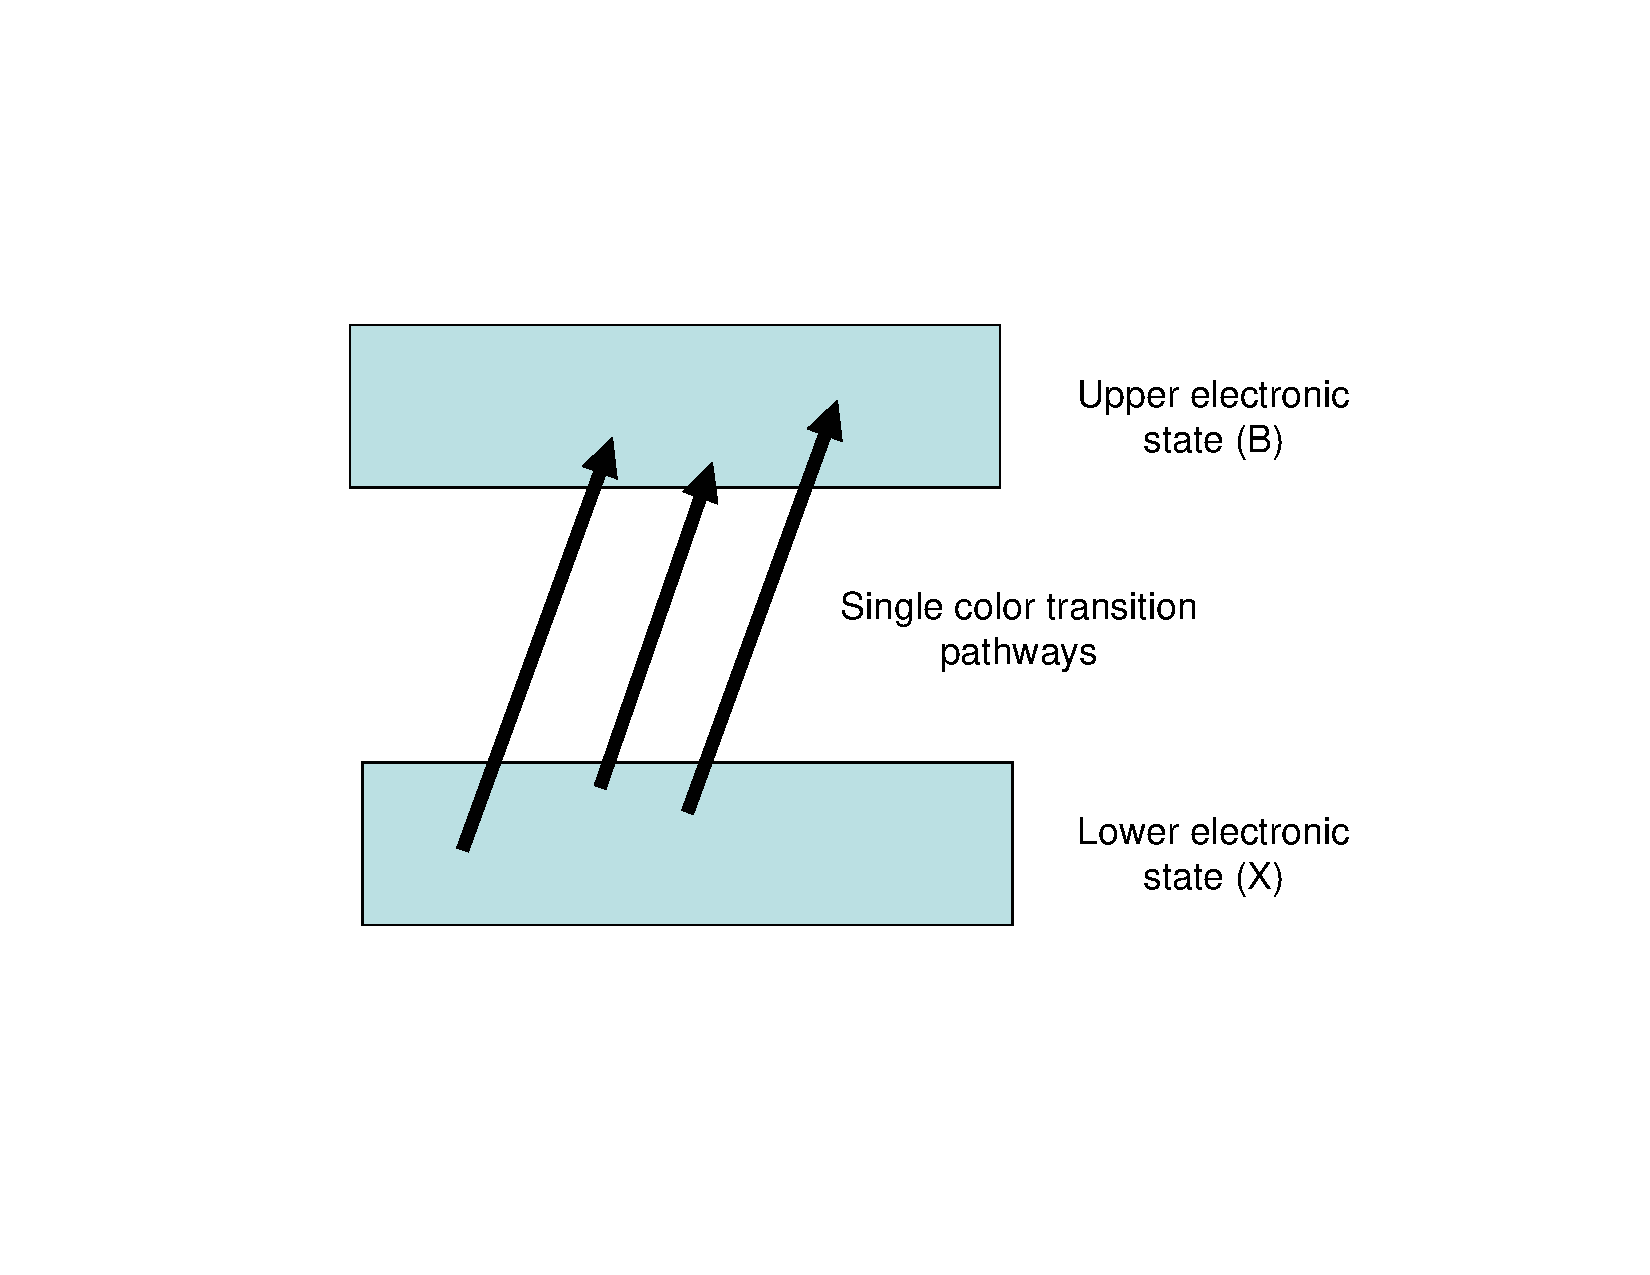
\includegraphics[bb=35 125 489 450]
{pathways_single/pathways_single.pdf}
}
\caption[Single transition diagram]{Single transition diagram. The upper and lower electronic states have a relatively dense substructure of ro-vibrational levels between which we induce transitions.}
\label{pathways_single}
\end{figure}
%----------------------------------------------------------------------------

%----------------------------------------------------------------------------
%----------------------------------------------------------------------------
%----------------------------------------------------------------------------
%bb defines the bounding box for the pdf
%viewport defines the area of the pdf used
%in sidewaysfigure the last entry in bb moves the caption toward/away the pic
%in sidewaysfigure the second entry in bb moves the pic toward/away the caption
%----------------------------------------------------------------------------
\begin{figure}
\scalebox{0.6}[0.6]{
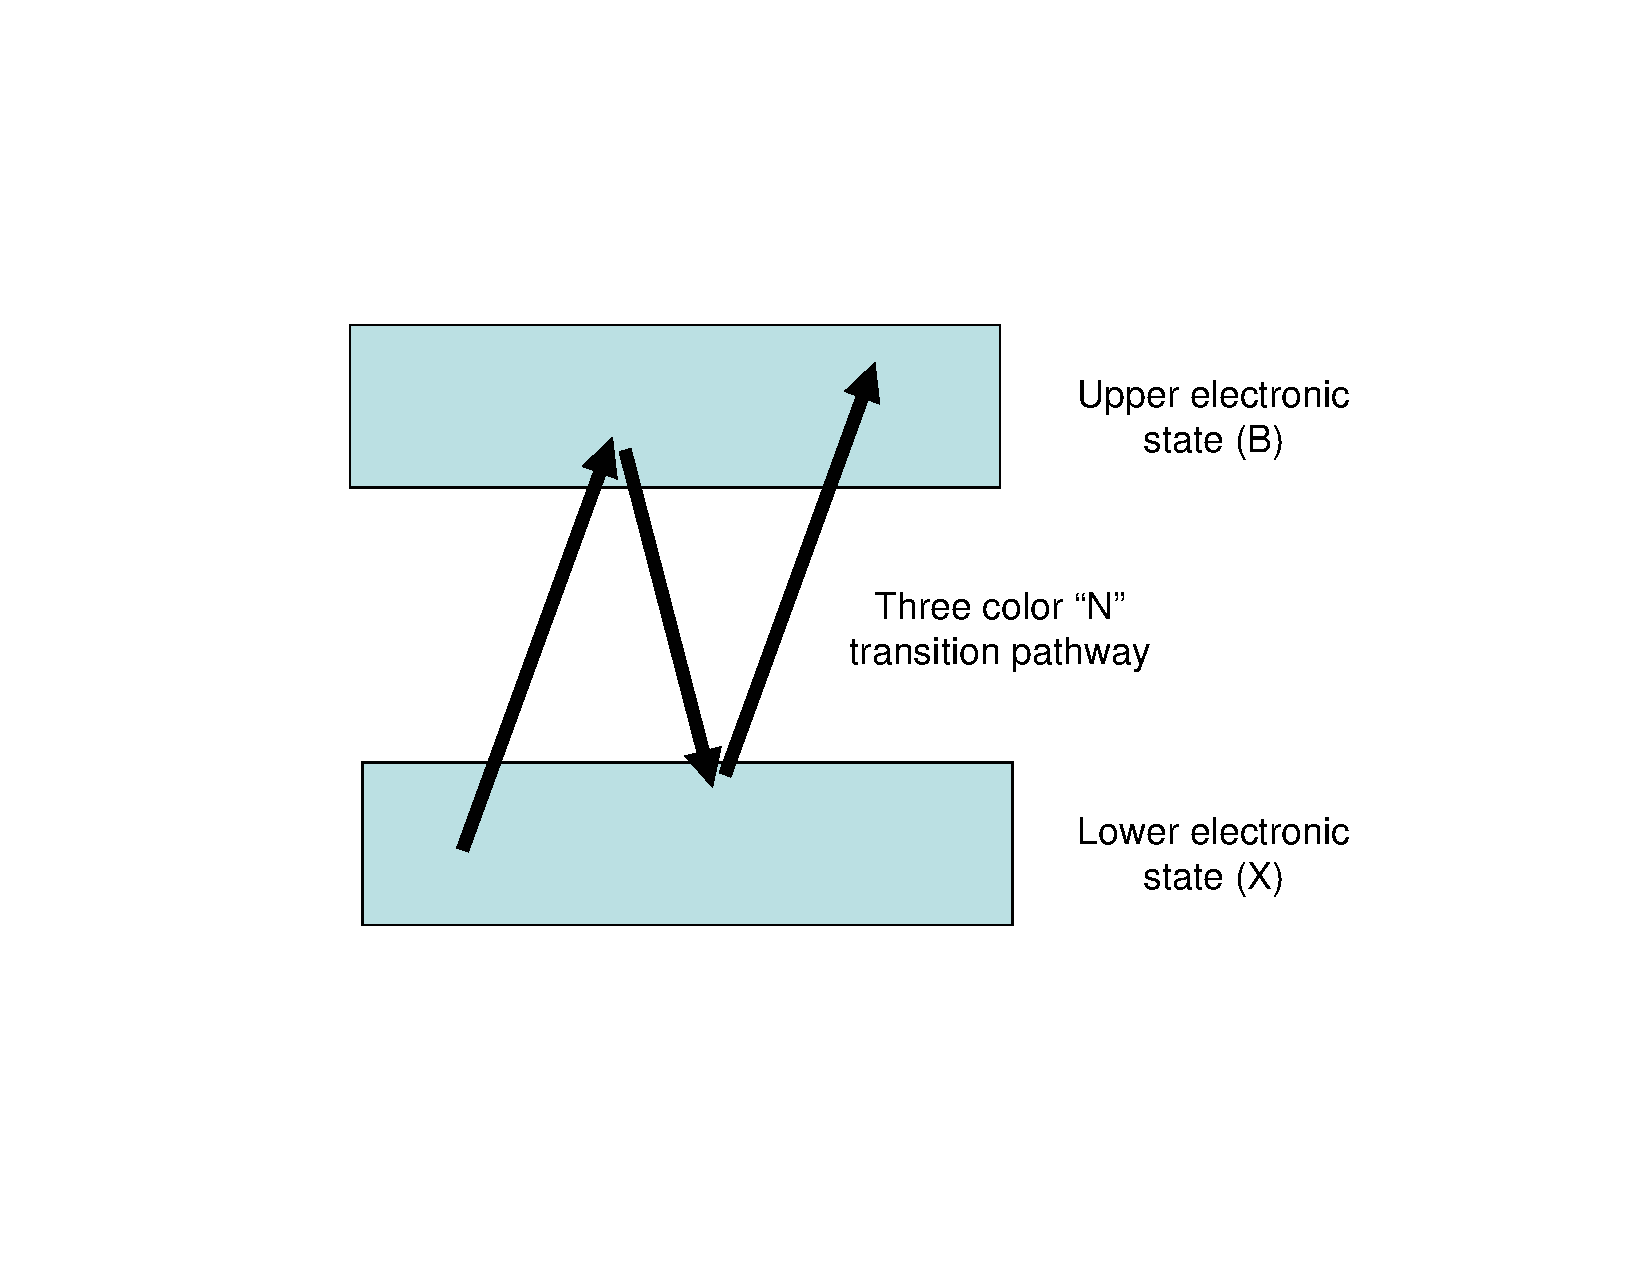
\includegraphics[bb=35 125 489 450]
{pathways_N/pathways_N.pdf}
}
\caption[``N'' transition diagram]{``N'' transition diagram.}
\label{pathways_N}
\end{figure}
%----------------------------------------------------------------------------

%----------------------------------------------------------------------------
%----------------------------------------------------------------------------
\begin{equation}
P(J^{\prime\prime},\nu^{\prime\prime},J^{\prime},\nu^{\prime})
=
L^{\prime}(J^{\prime\prime},\nu^{\prime\prime},J^{\prime},\nu^{\prime})
FCF(\nu^{\prime\prime},\nu^{\prime})
Boltz(\nu^{\prime\prime},\nu^{\prime})
\label{main approx}
\end{equation}
%----------------------------------------------------------------------------
where $L^{\prime}$ is from Equation \ref{norm lorentzian} (in Equation \ref{main approx} $L^{\prime}$ is interpreted as the detuning lineshape for non-resonant excitation; however, in Section \ref{tail} it was used to describe the rate at which fluorescence energy decreases with respect to detuning of the observed spectral window -- same line shape but different process), $FCF$ is the Franck-Condon factor, and $Boltz$ is the normalized Boltzmann probability for population of the lower state (i.e. the probability that the randomly selected molecule occupies the lower state of the transition of interest). In this way we obtain an estimate on the distribution of excited upper states due to single color excitation.

For a three color process (tuned to the target molecule), the second color's effect is treated much the same way except the upper B state becomes the ``source'' for the population transfer. Instead of the $Boltz$ factor we use the $P$'s from the first color; in short, the ensemble of states ``pulled'' up from the X state are ``pushed'' back down to the X state by the second color. Now the third color ``pulls'' this ensemble back up to the B state. In this way we obtain an estimate of the distribution of excited upper states due to three color excitation through a designed resonant pathway (an ``N'' transition).

The goal here is to create a unique population inversion in the target molecule which will glow in the green, while non-targets will glow red. In addition to the resonant pathway described above, there are many pathways one would have to average to gain a good estimate of the actual distribution of the upper states when using an approximation of this type. (The alternative is to track them with Equation \ref{dim eom}.) For the purposes of this argument, we will only compare the resonant pathway to the single color pathway. To support this assumption, the pathway is selected such that the second color pushes the resonant ensemble to an empty region of the X band. In our model we have FCFs for transitions involving lower states with vibrational quantum numbers up to 30: the energy for the X state with $\nu^{\prime\prime}=30$ and $J=0$ is 5916.8561 cm$^{-1}$, more than 29 times kT; so selecting an empty region of the X state is relatively easy.

%----------------------------------------------------------------------------
%----------------------------------------------------------------------------
